\chapter{HASIL DAN PEMBAHASAN}

% Ubah bagian-bagian berikut dengan isi dari pengujian dan analisis

Pada bab ini dipaparkan hasil dan analisa dari pelaksanaan skenario tahap  metodologi, skenario pengujian dan evaluasi pengujiannya. Pengujian dan evaluasi dilakukan guna mengetahui tingkat kesalahan dalam metodologi serta ananlisis untuk mencapai kesimpulan. Tahapan skenario yang dilaksanakan sebagai berikut :

% \begin{enumerate}
%   \item Pengujian akurasi model dalam beberapa situasi
%   \item Pengujian interaksi model pada beberapa responden
%   \item Pengujian pada robot dengan beberapa kondisi
% \end{enumerate}
% Dengan hasil metodologi serta pelaksanaan skenario-skenario pengujian yang dipaparkan pada bab Penelitian dan pembahasan, diharapkan mendapatkan hasil dan analisa sehingga dapatditarik kesimpulan dari pelaksanaan tugas akhir ini.

% \section{Hasil metodologi}
% Pada metodologi terdapat blok diagaram sebagai acuan dalam Penelitian yang telah dilaksanakan. Adapun hasil dari blok diagram tersebut secara rinci sebagai berikut :

\section{Skenario Dataset}

\begin{table}[H]
  \centering
  \caption{Citra hasil dataset}
  \label{tab:citradaset}
  \begin{tabular}{|c|c|c|c|}
  \hline
  Pose   & Citra & Pose   & Citra \\ \hline
  Diam   & 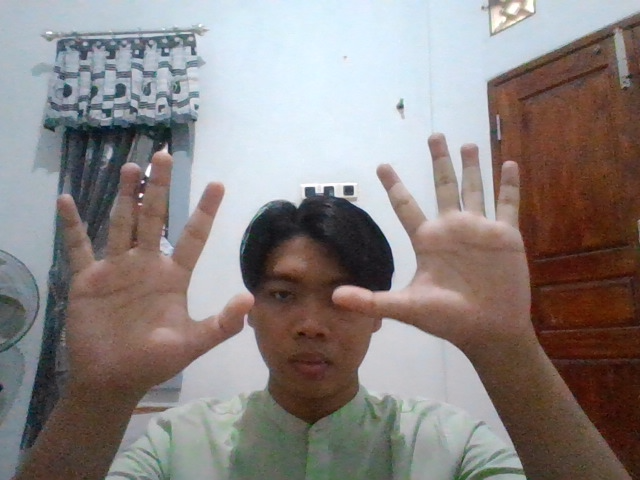
\includegraphics[width=0.3\linewidth]{../Gambar/posediam.png} &
  Kanan  & 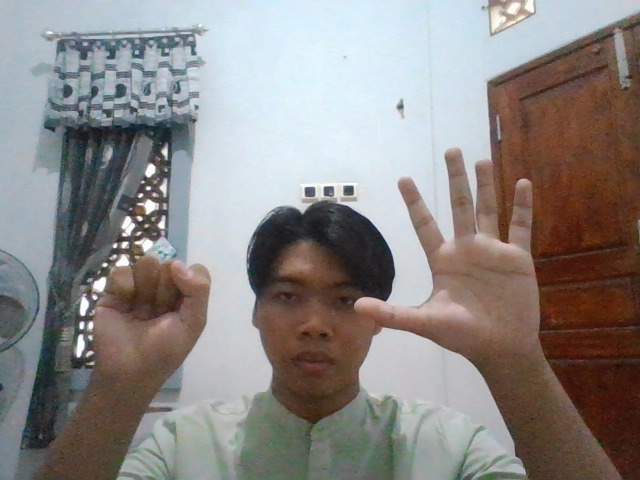
\includegraphics[width=0.3\linewidth]{../Gambar/posekanan.png} \\ \hline
  Kiri   & 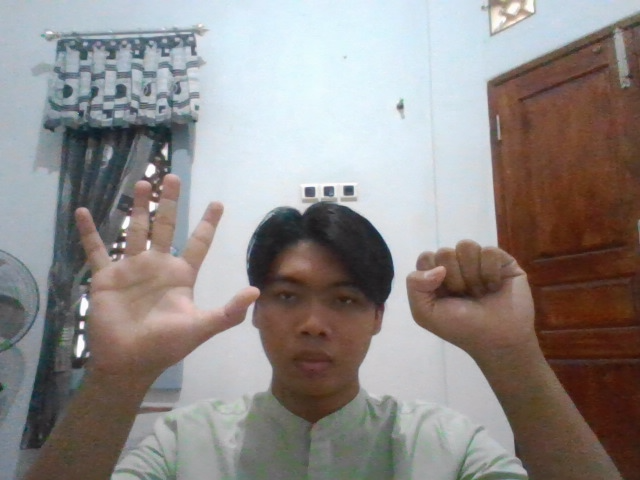
\includegraphics[width=0.3\linewidth]{../Gambar/posekiri.png} &
  Maju   & 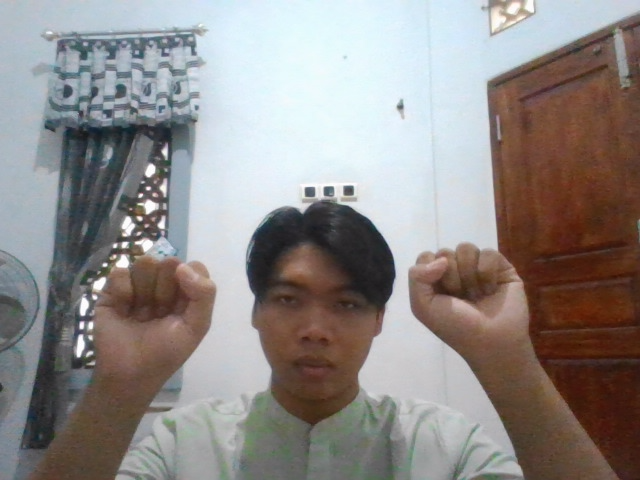
\includegraphics[width=0.3\linewidth]{../Gambar/posemaju.png} \\ \hline
  Mundur & 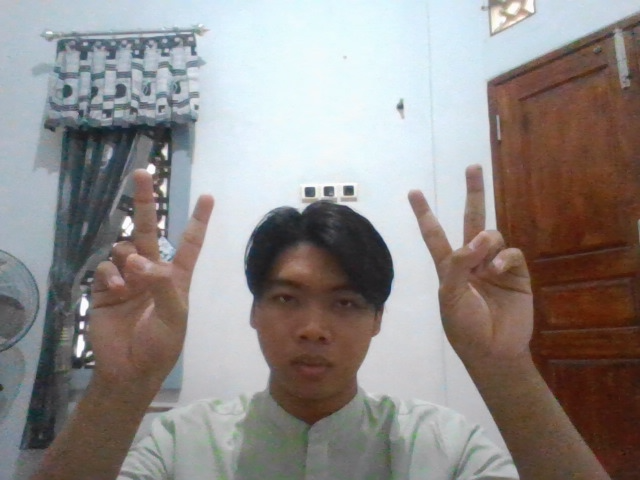
\includegraphics[width=0.3\linewidth]{../Gambar/posemundur.png} &
  Tembak & 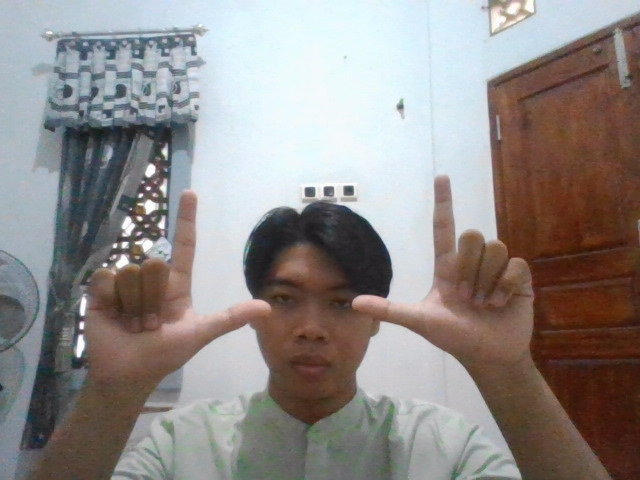
\includegraphics[width=0.3\linewidth]{../Gambar/posetembak.png} \\ \hline
\end{tabular}
\end{table}

Proses pengumpulan dataset dilakukan dengan pengambilan citra menggunakan kamera. Proses tersebut dilakukan selama beberapa waktu untuk dapat mendapatkan beberapa frame citra untuk suatu class dan diulang kembali dengan class yang berbeda sampai seluruh class terpenuhi. Seluruh citra tangan diambil dari satu orang yang sama dan menggunakan jarak pengambilan yang sama, yaitu jarak antara kamera dan tangan. Dalam proses pengambilan citra dilakukan beberapa variasi dalam pose tangan yaitu dengan sedikit merotasikan tangan dan sedikit melemaskan tangan. Hal ini dilakukan agar tiap class memiliki variasi pose dan dapat mendeteksi dari berbagai kondisi pose. Adapun pose yang digunakan sebagai dataset dapat dilihat pada Tabel \ref{tab:citradaset}.



\section{Skenario Pose \emph{Prediction}}

\begin{figure}[H]
  \centering
  \begin{tabular}{cc}
    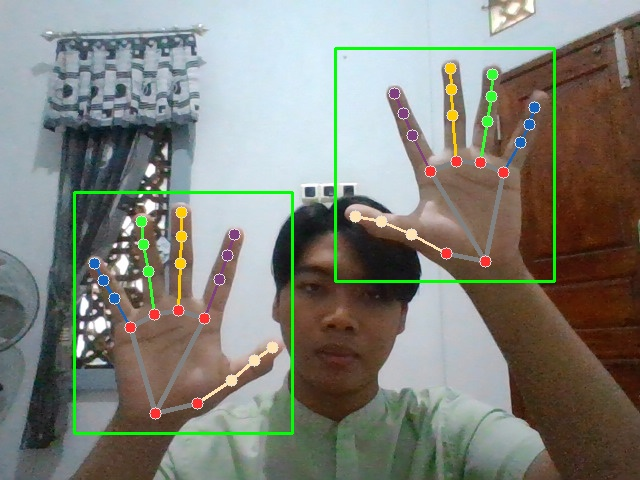
\includegraphics[width=0.4\linewidth]{../Gambar/hasilposepred.jpg} & 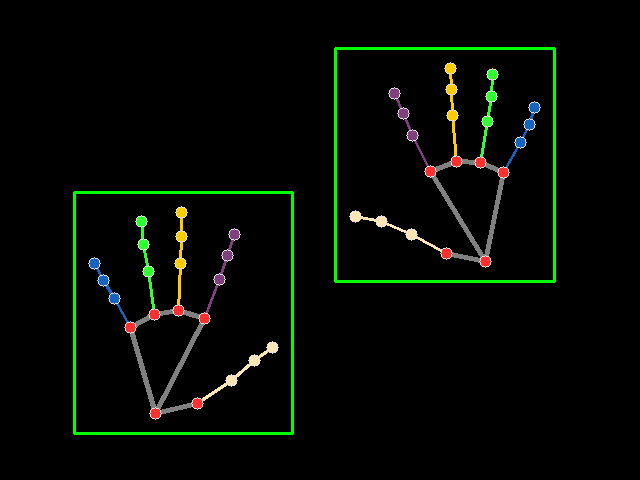
\includegraphics[width=0.4\linewidth]{../Gambar/hasilposepredhitam.png} \\
    a. Citra berwarna & b. Citra hitam 
    \end{tabular}
    \caption{Hasil\emph{ hand landmark}}
  \label{fig:hasilposepred}
\end{figure}

Proses pose \emph{prediction} dilakukan dengan menggambar \emph{hand landmark} yang telah terdeteksi dengan menggunakan \emph{Mediapipe} pada tiap-tiap citra yang telah dikumpulan pada tahap sebelumnya. Setelah \emph{hand landmark} tergambar maka tiap-tiap \emph{hand landmark} digambar pada citra berlatar gelap. Hasil dari \emph{hand landmark} pada citra hasil kamera dan citra hitam dapat dilihat pada Gambar \ref{fig:hasilposepred}. \emph{Hand landmark} yang terdapat pada citra ini diberikan \emph{bounding box} pada tiap tangan. Setelah \emph{bounding box} terbuat maka selanjutnya dilakukan \emph{hand localization} pada \emph{hand landmark} yang berada pada citra hitam. \emph{Hand} \emph{localization} ini untuk mengecilkan ukuran citra menjadi hanya selebar \emph{bounding box} dengan ditambah 20 \emph{pixel} pada nilai maksimal dan dikurangi 20 \emph{pixel} pada nilai minimum pada tiap \emph{bounding box}. Penambahan \emph{pixel} ini dimaksudkan untuk mencakup semua \emph{hand landmark} yang telah dibuat \emph{Mediapipe}. Dengan mengurangi ukuran citra ini bertujuan mengurangi waktu training dan dapat meningkatkan performa. Citra diluar \emph{bounding box} dibuang dan tiap \emph{bounding box} dirubah ukurannya menjadi 128x128 \emph{pixel} untuk menyamakan kedua \emph{bounding box} dalam satu frame citra. Setelah setiap ukuran \emph{bounding box} sama maka setiap \emph{bounding box} ditumpuk secara horizontal. Citra yang disimpan dan dijadikan dataset adalah citra yang terdapat dua \emph{hand landmark} yang telah ditumpuk secara horizontal. Citra yang disimpan nantinya memiliki ukuran 256x128 \emph{pixel} dikarenakan hasil dari dua tangan yang terdeteksi. Pada tahap menumpuk citra terdapat dua macam tumpukan yaitu citra dengan posisi tangan kiri berada pada kotak sebelah kiri dan tangan kanan pada kotak sebelah kanan. Posisi kedua yaitu tangan kiri berada pada posisi kanan dan tangan kanan berada pada kiri yang selanjutnya disebut sebagai posisi invers. Posisi \emph{hand landmark} dari hasil hand localization dapat dilihat pada Tabel \ref{tab:posisigtangan}.

\begin{table}[H]
  \centering
  \caption{Hasil posisi hand localization}
  \label{tab:posisigtangan}
  \begin{tabular}{|c|c|c|}
  \hline
  Pose   &Pose Benar&Pose Invers\\ \hline
  Diam   & 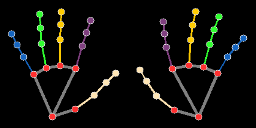
\includegraphics[width=0.3\linewidth]{../Gambar/Diam (1).png} & 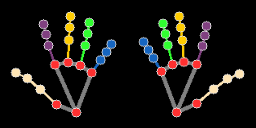
\includegraphics[width=0.3\linewidth]{../Gambar/DiamI (1).png} \\ \hline
  Kanan  & 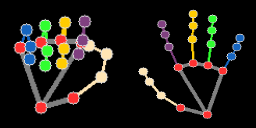
\includegraphics[width=0.3\linewidth]{../Gambar/Kanan (1).png} & 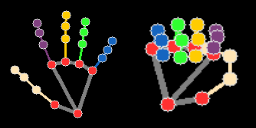
\includegraphics[width=0.3\linewidth]{../Gambar/KananI (1).png} \\ \hline
  Kiri   & 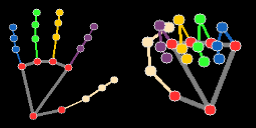
\includegraphics[width=0.3\linewidth]{../Gambar/Kiri (1).png} & 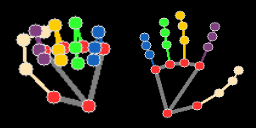
\includegraphics[width=0.3\linewidth]{../Gambar/KiriI (1).png} \\ \hline
  Maju   & 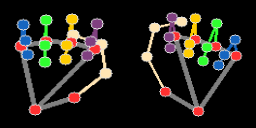
\includegraphics[width=0.3\linewidth]{../Gambar/Maju (1).png} & 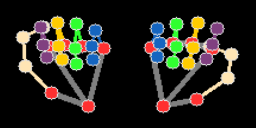
\includegraphics[width=0.3\linewidth]{../Gambar/MajuI (1).png} \\ \hline
  Mundur & 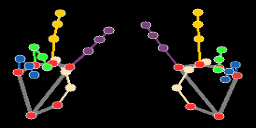
\includegraphics[width=0.3\linewidth]{../Gambar/Mundur (1).png} & 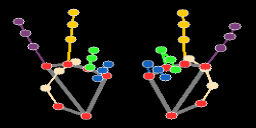
\includegraphics[width=0.3\linewidth]{../Gambar/MundurI (1).png} \\ \hline
  Tembak & 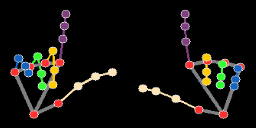
\includegraphics[width=0.3\linewidth]{../Gambar/Tembak (1).png} & 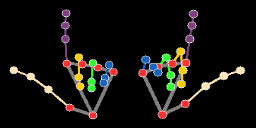
\includegraphics[width=0.3\linewidth]{../Gambar/TembakI (1).png} \\ \hline
  \end{tabular}
\end{table}




\section{Seknario Klasifikasi}
Proses klasifikasi dimulai dari \emph{training} dataset. Sebelum melakukan \emph{training} maka dibutuhkannya data citra pada tiap class. Tiap class memiliki \emph{train data} dan \emph{validation data}. Data-data ini diambil dari proses sebelumnya yaitu citra yang telah melewati tahap hand localization. Citra untuk train data pada tiap class berjumlah 400 dengan rincian 200 citra posisi benar dan 200 citra posisi invers, sedangkan citra untuk \emph{validation data} berjumlah 80 citra dengan 40 citra posisi benar dan 40 citra posisi invers. Adapaun tabel pesebaran data citra tiap class dapat dilihat pada Tabel \ref{tab:tiapclass}. \emph{Training} ini menggunakan CNN dengan menggunakan satu layer \emph{convolution} ukuran 3x3 dengan filter 16, sehingga ukuran citra yang awalnya 256x128 turun menjadi 254x126 yang disebabkan dari adanya konvolusi. Selanjutnya dilakukan \emph{pooling} dengan menggunakan \emph{max} \emph{pooling} ukuran 2x2 yang menyebabkan ukuran citra turun menjadi setengah dari hasil konvolusi yaitu 167x63. Layer selanjutnya yaitu \emph{flatten} dimana citra hasil dari max pooling di ubah menjadi vektor. Output yang didapatkan dari layer \emph{flatten} yaitu 128016 vektor.  Setelah di tentukannya konfigurasi layer CNN maka tahapan selanjutnya yaitu konfigurasi hyperparameter. Adapun konfigurasi pada hyperparameter yang digunakan dapat dilihat pada Tabel \ref{fig:hyperparameter} berikut. Citra yang digunakan sebagai data pada saat \emph{training} dan \emph{validation} berukuran 256x128 yang merupakan citra hasil ekstraksi fitur. Jumlah total dari image yang digunakan untuk \emph{training} berjumlah 2400 citra. 2400 citra tersebut tidak memungkingkan untuk langsung di \emph{training} pada sekali \emph{epoch} maka dari itu citra dibagi menjadi beberapa step per epoch dan \emph{batchsize}. Tiap step per epoch akan menggunakan 32 citra, jumlah step per epoch ini selanjutnya dipanggil sebagai \emph{batchsize}. Alasan penggunaan batchsize dengan nilai 32 untuk mengurangi beban pada laptop pada saat dilakukan \emph{training}. Tiap step per epoch menggunakan 32 citra maka dibutuhkan 75 step per epoch pada sekali \emph{epoch}, 75 step per epoch ini selanjutnya di sebut sebagai step per epoch.

\begin{table}[H]
  \centering
  \caption{Jumlah Citra Tiap \emph{Class}}
  \label{tab:tiapclass}
  \begin{tabular}{|c|c|c|}
  \hline
  \emph{Class}  & Train Data & Validation Data \\ \hline
  Diam   & 400        & 80              \\ \hline
  Kanan  & 400        & 80              \\ \hline
  Kiri   & 400        & 80              \\ \hline
  Maju   & 400        & 80              \\ \hline
  Mundur & 400        & 80              \\ \hline
  Tembak & 400        & 80              \\ \hline
  \end{tabular}
\end{table}

\begin{table}[H]
  \centering
  \caption{Konfigurasi \emph{hyperparameter}}
  \label{fig:hyperparameter}
  \begin{tabular}{|c|c|lll}
  \cline{1-2}
  \emph{Hyperparameter} & Konfigurasi \\ \cline{1-2}
  Epochs         & 10 \\ \cline{1-2}
  Batchsize      & 32 \\ \cline{1-2}
  Image Size     & 256x128 \\ \cline{1-2}
  Step per epoch      & 75 \\ \cline{1-2}
  Optimizer      & Adam \\ \cline{1-2}
  \end{tabular}
\end{table}

Setelah proses konfigurasi layer CNN dan \emph{hyperparameter} telah dilakukan. Selanjutnya yaitu proses \emph{training} yaitu berupa model dan detail data pada tiap proses pengulangan. Hasil dari \emph{training} ini didapatkan \emph{training} akurasi, \emph{validation} akurasi, \emph{training} \emph{loss}, dan \emph{validation} \emph{loss}. Setiap perulangan mendapatkan nilai tersebut, grafik dari nilai tersebut dalam 10 perulangan dapat dilihat pada Gambar \ref*{fig:loss} dan Gambar \ref*{fig:akurasi}. Dapat dilihat dari grafik \emph{training} akurasi bahwa pada epoch pertama nilai \emph{training} akurasi didapatkan 0.9 dan pada perulangan selanjutnya nilai akurasi stabil di angka 0.9. Pada grafik \emph{training loss} pada epoch pertama didapatkan nilai \emph{training loss} sebesar 0.2 dan semakin mengecil pada epoch selanjutnya. Pada epoch ke sepuluh didapatkan nilai \emph{training} akurasi 0.99 dan nilai \emph{training loss} 0.0036. 

\begin{figure}[H]
  \centering
  \includegraphics[width=0.7\linewidth]{../Gambar/loss.png}
  \caption{Grafik \emph{training} dan \emph{validation} \emph{loss}}
  \label{fig:loss}
\end{figure}

\begin{figure}[H]
  \centering
  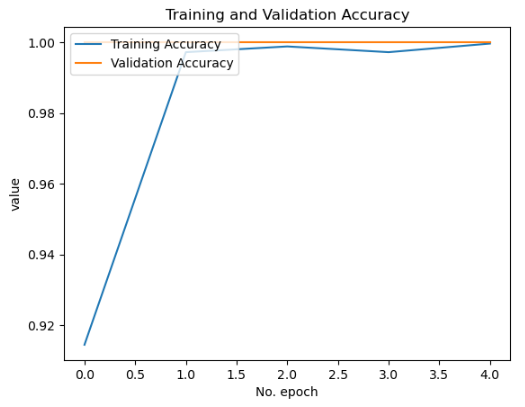
\includegraphics[width=0.7\linewidth]{../Gambar/akurasi.png}
  \caption{Grafik \emph{training} dan \emph{validation} akurasi}
  \label{fig:akurasi}
\end{figure}

Setelah proses \emph{training} selesai dan telah didapatkan model dengan akurasi yang tinggi atau sesuai \emph{threshold} dalam hal ini dapat dilihat pada grafik akurasi pada Gambar \ref{fig:akurasi}, maka selanjutnya masuk kepada proses evaluasi model. Evaluasi model menggunakan \emph{confusion matrix} dengan data testing citra sebanyak 100 pada masing-masing class. Hasil dari \emph{confusion matrix} didapatkan akurasi 0.99. Hasil evaluasi dengan \emph{confusion matrix} secara lengkap dapat dilihat pada Gambar \ref{fig:confusionmatrix}. Model yang telah dievaluasi menggunakan \emph{confusion matrix} selanjutnya digunakan sebagai klasifikasi. Klasifikasi menghasilkan kode instruksi yang digunakan sebagai acuan dalam memberikan perintah kepada robot. Adapun kode instruksi yang diatur sebagai perintah kepada robot dapat dilihat pada Tabel \ref{tab:kodeinstruksi}

\begin{figure}[H]
  \centering
  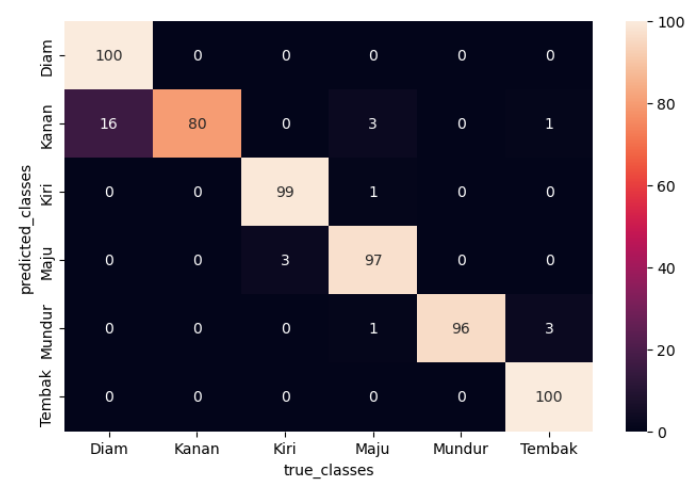
\includegraphics[width=0.7\linewidth]{../Gambar/confusionmatrix.png}
  \caption{Hasil \emph{Confusion Matrix}}
  \label{fig:confusionmatrix}
\end{figure}

\begin{table}[H]
  \centering
  \caption{Kode instruksi hasil klasifikasi}
  \label{tab:kodeinstruksi}
  \begin{tabular}{|c|c|}
  \hline
  Pose   & Kode Instruksi \\ \hline
  Diam   & n              \\ \hline
  Kanan  & r              \\ \hline
  Kiri   & l              \\ \hline
  Maju   & f              \\ \hline
  Mundur & b              \\ \hline
  Tembak & s              \\ \hline
  \end{tabular}
\end{table}

\section{Seknario Kontrol Navigasi}
Proses kontrol navigasi diawali dengan perancangan komunikasiantara laptop dengan robot dan dilanjutkan perancangan pada robot. Komuniasi antara laptop dengan robot menggunakan \emph{web socket}. Robot dirancang dengan memiliki kemampuan untuk bergerak dan menembak.  Kebutuhan robot dengan adanya kemampuan bergerak dan menembak membutuhkan mikrokontroler untuk mengatur semua itu dan juga untuk koneksi secara \emph{wireless} dengan laptop. \emph{Mikrokontroller} yang digunakan yaitu "nodeMCU ESP8266" dengan alasan sudah memiliki modul \emph{WiFi} yang terpasang didalamnya dan juga memiliki kemampuan yang cukup untuk dapat mengontrol robot. Pergerakan robot dapat terjadi dikarenakan adanya sepasang roda yang dipasangkan pada robot. Untuk menggerakkan roda pada robot dibutuhkan motordc yang dipasangkan pada roda. Motordc yang digunakan berjumlah dua buah yang dipasangkan pada robot. Motordc dapat menggerakkan roda ketika dialiri oleh arus listrik. \emph{Mikrokontroller} tidak dapat secara langsung mengatur aliran listrik yang masuk kepada motordc, maka dari itu dibutuhkannya \emph{motor driver}. Arus listrik yang akan mengalir ke motor dc akan diatur oleh motor driver. Semakin kuat arus listrik yang mengalir ke motor dc maka akan semakin cepat perputaran roda yang mengakibatkan semakin cepat pergerakan dari robot. Kemampuan menembak pada robot diatur dengan adanya sensor \emph{infrared}. Sensor \emph{infrared transmitter} diletakkan di depan robot sedangkan sensor \emph{infrared receiver} membutuhkan empat yang diletakkan disekeliling sisi robot. Sensor \emph{infrared transmitter} diletakkan di depan dengan tujuan saat menembak, arah tembakan robot ke depan searah dengan robot. Saat menembak robot terlebih dahulu dan kemudian mengaktifkan sensor \emph{infrared transmitter} sebagai simbol dari menembak. Saat menembak sensor \emph{infrared transmitter} akan mengirimkan pesan dalam bentuk \emph{hexadecimal} dan pada masing-masing robot akan memiliki nilai \emph{hexadecimal} yang berbeda. Sensor \emph{infrared receiver} di sambungkan secara pararel untuk ke empat sensornya dan dihubungkan kepada mikrokontroler. Sensor \emph{infrared receiver} diletakkan disekeliling dengan tujuan robot dapat tertembak dari segala arah. Saat sensor \emph{infrared receiver} menerima tembakan maka akan dicek terlebih dahulu pesan \emph{hexadecimal} yang diterima. Pesan yang diterima oleh sensor \emph{infrared receiver} dan sesuai dengan pesan \emph{hexadecimal} dari yang dikirim robot maka pesan terbesut dikirim kepada laptop melalu koneksi internet. Secara schematic dapat dilihat pada Gambar \ref{fig:schematic}.

\begin{figure}[H]
  \centering
  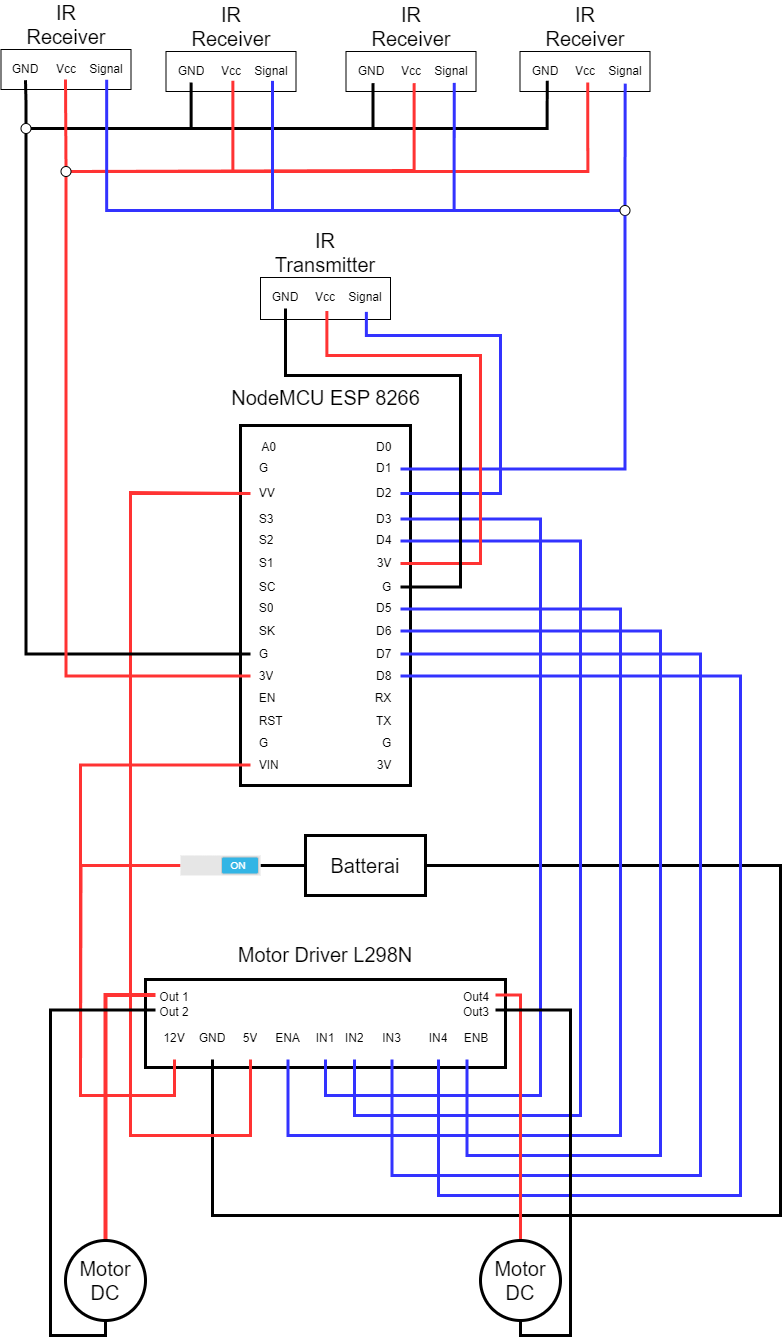
\includegraphics[width=0.5\linewidth]{../Gambar/schematic.png}
  \caption{\emph{Schematic} robot}
  \label{fig:schematic}
\end{figure}

\section{Seknario Pengujian Jarak Model}
Pengujian ini menggunakan tangan peneliti dengan variasi jarak tangan terhadap kamera. Pengujian jarak dilakukan untuk mengetahui jarak ideal dari model. Jarak yang dimaksud merupakan jarak antara kamera dengan  kedua tangan. Ketinggian dari tangan sejajar dengan kamera dan telapak tangan menghadap kepada kamera. Pengujian jarak dilakukan dengan cara mengambil 20 citra dari tiap \emph{class} pada jarak tertentu. Jarak ini dimulai dari 40cm, 60cm, dan 100cm antara tangan dengan kamera. Pengujian dilakukan karena adanya perubahan bentuk dari \emph{hand landmark} yang dipengaruhi oleh jarak. Hasil pose yang terdeteksi dari pengujian jarak dapat dilihat pada Tabel \ref{tab:hasiljarak} dan hasil confusion matrix dari masing-masing jarak dapat dilihat pada Gambar \ref{fig:confusionmatrixjarak}. Dari hasil pengujian didapatkan nilai akurasi tertinggi pada jarak 40 cm dan pada jarak 60cm didapatkan nilai 0.99, namun pada jarak 80cm dan 100cm akurasi menurun menjadi 0.92. Jarak 40cm dan 60cm memiliki akurasi tinggi dikarenakan jarak tersebut sama dengan jarak saat pengambilan dataset.

\begin{figure}[H]
    \begin{tabular}{cc}
      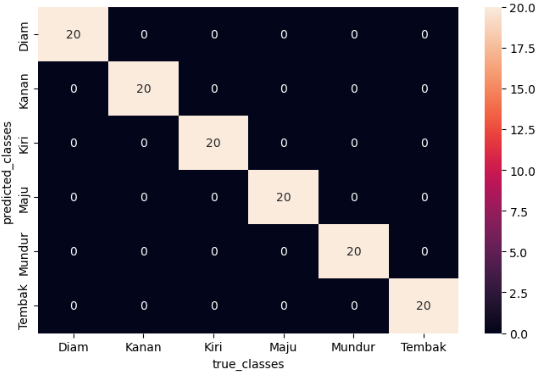
\includegraphics[width=0.5\linewidth]{../Gambar/cm30.png} & 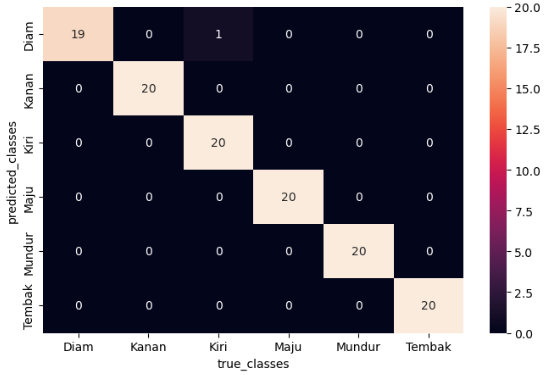
\includegraphics[width=0.5\linewidth]{../Gambar/cm50.png} \\
      a. Jarak 40cm & b. Jarak 60cm \\ 
      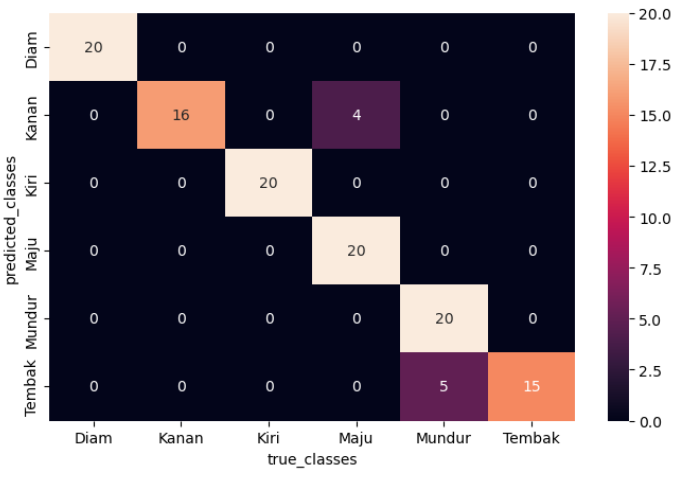
\includegraphics[width=0.5\linewidth]{../Gambar/cm80.png} & 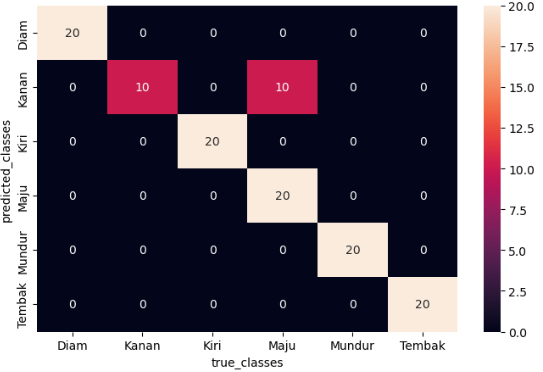
\includegraphics[width=0.5\linewidth]{../Gambar/cm100.png} \\
      c. Jarak 80cm & d. Jarak 100cm
    \end{tabular}
    \centering
    \caption{Pengujian \emph{Confussion Matrix} pada jarak tertentu}
    \label{fig:confusionmatrixjarak}
\end{figure}

\begin{table}[H]
  \centering
  \caption{Pose yang terdeteksi dari pengujian jarak}
  \label{tab:hasiljarak}
  \begin{tabular}{|c|clll|}
    \hline
    \multirow{2}{*}{Pose} & \multicolumn{4}{c|}{Jarak (cm)}                                                   \\ \cline{2-5} 
                          & \multicolumn{1}{l|}{40} & \multicolumn{1}{l|}{60} & \multicolumn{1}{l|}{80} & 100 \\ \hline
    Diam                  & \multicolumn{1}{c|}{20}   & \multicolumn{1}{l|}{19}   & \multicolumn{1}{l|}{20}   &   20  \\ \hline
    Kanan                 & \multicolumn{1}{c|}{20}   & \multicolumn{1}{l|}{20}   & \multicolumn{1}{l|}{10}   &   10  \\ \hline
    Kiri                  & \multicolumn{1}{c|}{20}   & \multicolumn{1}{l|}{20}   & \multicolumn{1}{l|}{20}   &   20  \\ \hline
    Maju                  & \multicolumn{1}{c|}{20}   & \multicolumn{1}{l|}{20}   & \multicolumn{1}{l|}{20}   &   20  \\ \hline
    Mundur                & \multicolumn{1}{c|}{20}   & \multicolumn{1}{l|}{20}   & \multicolumn{1}{l|}{20}   &   20  \\ \hline
    Tembak                & \multicolumn{1}{c|}{20}   & \multicolumn{1}{l|}{20}   & \multicolumn{1}{l|}{20}   &   20  \\ \hline
    Akurasi                  & \multicolumn{1}{c|}{1}   & \multicolumn{1}{l|}{0.99}   & \multicolumn{1}{l|}{0.92}   &   0.92  \\ \hline
  \end{tabular}
\end{table}


\section{Skenario Uji Pengaruh Sudut Kamera (DATA BELUM ADA)}
Pengujian sudut kamera dilakukan menggunakan tangan peniliti dengan jarak uji 40cm dari kamera dan bergeser 40cm dari kamera. Terdapat empat sudut yang akan diujikan yaitu kanan, kiri, bawah, dan atas. Pengujian ini dilakukan untuk mengatahui kemampuan model terhadap variasi posisi tangan yang tidak tepat didepan kamera, karena dataset yang digunakan tangan tepat berada didepan kamera. Data testing yang akan digunakan berjumlah 20 citra tiap \emph{class}. Hasil dari pengujian pengaruh sudut kamera terhadap model dapat dilihat pada Tabel

\begin{table}[H]
  \centering
  \caption{Pose yang terdeteksi dari pengujian sudut kamera}
  \label{tab:hasilsudut}
  \begin{tabular}{|c|clll|}
    \hline
    \multirow{2}{*}{Pose} & \multicolumn{4}{c|}{Posisi} \\ \cline{2-5} 
      & \multicolumn{1}{l|}{Kanan} & \multicolumn{1}{l|}{Kiri} & \multicolumn{1}{l|}{Atas} & Bawah \\ \hline
    Diam                  & \multicolumn{1}{c|}{20}   & \multicolumn{1}{l|}{19}   & \multicolumn{1}{l|}{20}   &   20  \\ \hline
    Kanan                 & \multicolumn{1}{c|}{20}   & \multicolumn{1}{l|}{20}   & \multicolumn{1}{l|}{10}   &   10  \\ \hline
    Kiri                  & \multicolumn{1}{c|}{20}   & \multicolumn{1}{l|}{20}   & \multicolumn{1}{l|}{20}   &   20  \\ \hline
    Maju                  & \multicolumn{1}{c|}{20}   & \multicolumn{1}{l|}{20}   & \multicolumn{1}{l|}{20}   &   20  \\ \hline
    Mundur                & \multicolumn{1}{c|}{20}   & \multicolumn{1}{l|}{20}   & \multicolumn{1}{l|}{20}   &   20  \\ \hline
    Tembak                & \multicolumn{1}{c|}{20}   & \multicolumn{1}{l|}{20}   & \multicolumn{1}{l|}{20}   &   20  \\ \hline
    Akurasi                  & \multicolumn{1}{c|}{1}   & \multicolumn{1}{l|}{0.99}   & \multicolumn{1}{l|}{0.92}   &   0.92  \\ \hline
  \end{tabular}
\end{table}

\begin{figure}[H]
    \begin{tabular}{cccc}
      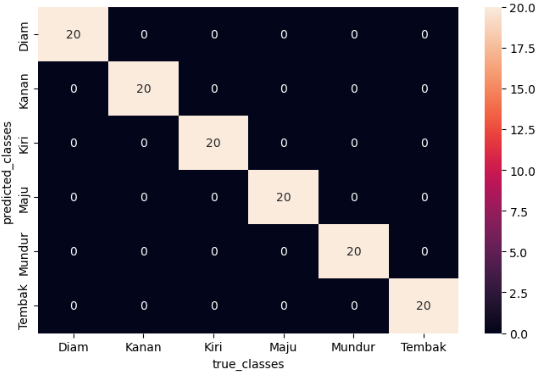
\includegraphics[width=0.4\linewidth]{../Gambar/cm30.png} & 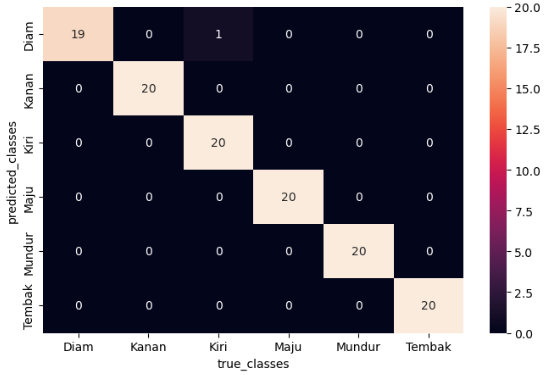
\includegraphics[width=0.4\linewidth]{../Gambar/cm50.png} \\
      a. Jarak 40cm & b. Jarak 60cm \\ 
      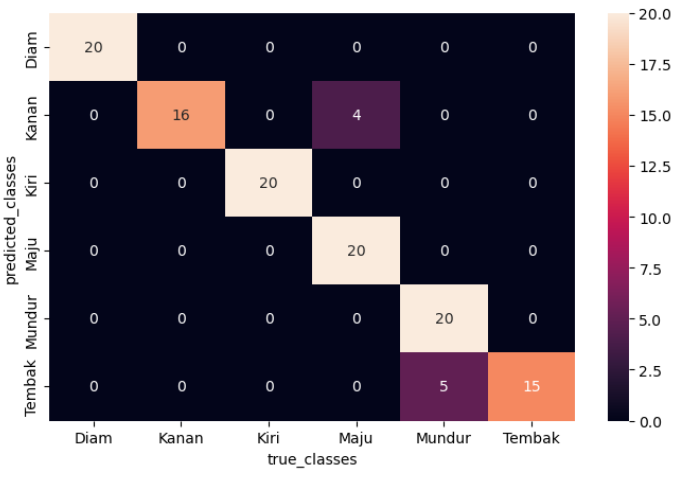
\includegraphics[width=0.4\linewidth]{../Gambar/cm80.png} & 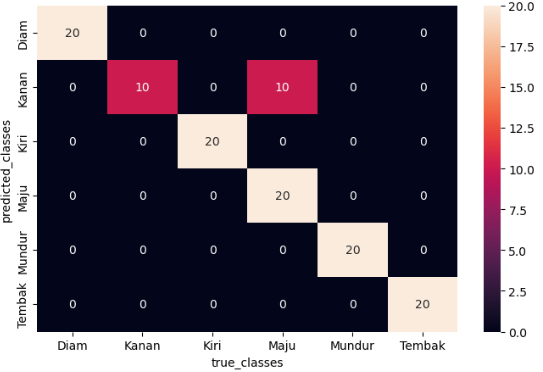
\includegraphics[width=0.4\linewidth]{../Gambar/cm100.png} \\
      c. Jarak 80cm & d. Jarak 100cm
    \end{tabular}
    \centering
    \caption{Pengujian \emph{Confussion Matrix} pada jarak tertentu}
    \label{fig:cmsudut}
\end{figure}

\section{Skenario Uji Pengaruh Instensitas Cahaya}


\section{Skenario Uji Jarak Komunikasi (DATA KURANG)}
Robot yang telah dirancang selanjutnya diuji dengan cara mengirimkan kode instruksiyang dihasilkan dari proses klasifikasi kepada mikrokontroler robot. Pengujian ini dilakukan dengan mengklasifikasi 20 citra pada tiap \emph{class}. Pengujian ini bertujuan untuk mengetahuiapakah ada data yang tidak terkirim atau hilang saat dikirim. Hasil dari klasifikasi akan dirubah menjadi kode instruksi dan dikirim kepada mikrokontroler. Pada mikrokontroler dihitung jumlah kode instruksi yang masuk dan dibandingkan dengan kode yang dikirim. Hasil pengujian ini dapat dilihat pada Tabel \ref{tab:hasulujipose}

\begin{table}[H]
  \centering
  \caption{Hasil uji komunikasi laptop dengan robot}
  \label{tab:hasulujipose}
  \begin{tabular}{|c|c|}
  \hline
  Pose   &  Hasil Uji\\ \hline
  Diam   & 20              \\ \hline
  Kanan  & 20             \\ \hline
  Kiri   & 20              \\ \hline
  Maju   & 20              \\ \hline
  Mundur & 20              \\ \hline
  Tembak & 20              \\ \hline
  \end{tabular}
\end{table}

  % \item Pengujian intensitas cahaya \\
  % Pengujian intensitas cahaya 
  % \item Pengujian sudut kamera \\